\newif\ifdraft
\ifx\dontdraft\relax
\message{IFX TRUE}
\draftfalse
\else
\message{IFX FALSE}
\drafttrue
\fi
% Final version: use times!
% \documentstyle[times,graphicx,ht01e]{article}
\documentstyle[isolatin1,times, concmath,uist, graphicx]{article}
% \draftfalse

\ifdraft
\renewcommand{\baselinestretch}{0.9}
\def\margincomment#1{
\marginpar{
\vbox{
\scriptsize #1
}
}}
\def\nakki#1{\marginpar{\bf Nakki: #1}}
\pagestyle{plain}
\else
\def\margincomment#1{}
\def\nakki#1{}

% Make the times fonts defaults again if not draft.
\renewcommand{\sfdefault}{phv}
\renewcommand{\rmdefault}{ptm}
\renewcommand{\ttdefault}{pcr}

\fi


% Define a macro for your own margin notes here
% If it is ABSOLUTELY clear that something is a typo, go ahead
% and fix it. But don't make any major changes to the text itself
% yet. Also, only propose rearrangements in the margin: CVS doesn't
% work too well with rearrangements and edits done by several
% people. I will be the editor until wed or thu.
\def\tjl#1{\margincomment{Tjl: #1}}
\def\vp#1{\margincomment{vp: #1}}
\def\rr#1{\margincomment{rr: #1}}
\def\cat#1{\margincomment{cat: #1}}
\def\ajk#1{\margincomment{ajk: #1}}
\def\jvk#1{\margincomment{jvk: #1}}
\def\benja#1{\margincomment{benja: #1}}



% \documentstyle[times,graphicx,uist,isolatin1]{article}
\begin{document}

\newcommand{\url}[1]{\textsf{#1}}
\newcommand{\hyp}{\discretionary{}{}{}}


\bibliographystyle{plain}
\title{
%Decoupling views from enhancements;
Vobs: a framework for pervasive animation/morphing and connectivity
%a fourth tier for MVC
}

%%
%% Note on formatting authors at different institutions, as shown below:
%% Change width arg (currently 7cm) to parbox commands as needed to
%% accommodate widest lines, taking care not to overflow the 17.8cm line width.
%% Add or delete parboxes for additional authors at different institutions. 
%% If additional authors won't fit in one row, you can add a "\\"  at the
%% end of a parbox's closing "}" to have the next parbox start a new row.
%% Be sure NOT to put any blank lines between parbox commands!
%%

\author{
\parbox[t]{8.9cm}{\centering
             {\em Tuomas J. Lukka, Vesa Parkkinen, Rauli Ruohonen}\\
  Dept.~of Mathematical Information Technology\\
  University of Jyv\"askyl\"a, PO.~Box~35\\
  FIN-40351~Jyv\"askyl\"a\\
  Finland\\
  \{lukka,veparkki,raulir\}@iki.fi}
\parbox[t]{8.9cm}{\centering
             {\em Benjamin Fallenstein}\\
  Oberstufen-Kolleg\\
  University of Bielefeld\\
  PO.~Box~100131, D-33501 Bielefeld\\
  Germany\\
  b.fallenstein@gmx.de}
}

\maketitle

\ifdraft
\textwidth 6.6cm
\columnwidth 8.6cm
\onecolumn
% \textwidth 8.5cm
\marginparwidth 8.5cm
\fi

\abstract

\benja{
(currently about 130 words out of a maximum of 199; this should probably get
a bit wordier so that we explain as clearly as possible.)
}
\tjl{XXX How much now?}
\benja{ARGH. About 260. More that 25\% above what they're ok with.}
\tjl{Not a problem. We'll cut it down.}

We introduce the goal of pervasive animation/morphing and connectivity:
different visual representations of the same underlying ``object''
should always be visually connected, either by drawing a
connecting line or other graphic, or (if shown at different times)
by animating from one to the other.

While animation has been used in computing for a long time,
animations are, with few exceptions, achieved either by 
modifying a continuous
view parameter and redrawing or using previously drawn ``canned''
animations. 

This inherently couples the animation to a single view of the data,
which we argue is too restrictive.
The same data can be viewed through several different views,
and the views should be decoupled
from the animation: explicit programming should
not be required for
 morphing or connecting between two views developed independently.

To provide this functionality,
we introduce the Vob system, a medium-level representation 
%suitable for focus+context and other
which easily allows animation and showing connections between different
views. 
Instead of drawing directly to the screen, 
the views split their output into parts corresponding to different
underlying ``objects'', which are then rendered onto the screen. 
The system does not limit the graphical expression of the views,
since the parts can render themselves in any way they like, but simply
attaches some semantic information to the scene.
This allows the Vob system to provide a crude but effective
animation between independent views.

%We also discuss the use of the Xanadu media model in connection with vobs in
%order with vobs in order to show connections between different copies of
%the same piece of media easily. 

Our system can be seen as a fourth tier to the commonly used three-tier
MVC (Model-View-Controller) pattern. 
\tjl{Can't find a reasonable place for the MVC mention.}

Finally, we discuss our prototype Java implementation of the Vob system
and examples implemented using it.
\benja{We need to say somewhere
that we are explaining an actually implemented system. See UIST author's
guidelines.}



\keywords Focus+context, medium-level representation, animation, 
    connections, Xanadu media model

% \tolerance=400 
\tolerance=500 
  % makes some lines with lots of white space, but      
  % tends to prevent words from sticking out in the margin

\def\vob{{\tt Vob}}
\def\vobscene{{\tt VobScene}}
\def\view{{\tt View}}
\def\key{{\tt key}}
\def\diff{{\tt diff}}

\def\unfin{\tiny}
\def\fin{\normalsize}

\section{INTRODUCTION}

One of the earliest mockups of windowed systems, published by
Ted Nelson in 1972\cite{as-we-will-think},
includes graphical connections between related information
in two side-by-side documents.
A more recent recent discussion can be found in 
\cite{ted-xanalogical-structure-needed}.
Such awareness of interconnectedness has only rarely been
incorporated into production or prototype UIs; for 
a good example where interconnections {\em are} shown inside
one spreadsheet, see \cite{igarashi98fluid}.

In this article, we present the Vob system
which is a new layer to the three-tier Model-View-Controller\cite{XXX}
model enabling pervasive animation and interconnections between 
different views of the same data.

The following sections first introduce our concept of pervasive animation
and interconnectivity, discuss the Vob system, discuss the GZigZag 
system as an example of its use, as well as another example, the file browser.
Subsequently, we look at th Xanadu media model and the generalization of
the Vob system to handle that, and the availability of the prototype 
implementation.

\unfin

The Model-View-Controller\cite{XXX} paradigm is an age-tested
technique for showing several views of the same, changing data.
The fundamental idea is to define an object-oriented structure
where the underlying Model informs the Views showing parts of it
about changes in a uniform manner.

Model-View-Controller\cite{XXX} is geared towards the conventional
windowing systems where the different views are fixed to their respective
windows. 
In such systems, connections between data in different windows
are conventionally not shown ... 
Nelson's early mockups + microcosm demo

N�kym�t, monoliittiset systeemit

Samat asiat useissa n�kymiss� esim: file manager - 
    lista ja ikonin�kym�, hakemistot sek� puussa ett� ikoneissa.
    IMPLEMENTAATIO?

Sama teksti useissa versioissa tiedostoa vierekk�in - insufficiency
off \diff.

Ref: spread-sheet which shows connections (cell references etc.) of cells
    near the mouse cursor.

Self (chang), artkit
Lasseter 87
NEED MORE INFORMATION ON SELF!

Animation is widely used in today's graphical user interfaces.
The particular uses, however, are specialized and each use of animation
has been separately designed. XXX Refs.

The basic idea of the Vob system is to create a medium-level
representation of the view which can be used to allow animation
or connections to be shown between wildly different visualizations.

Scientific animations?

Windows popping out from icons!!! Animations clarifying the relations
of things.

\fin

\section{PERVASIVE ANIMATION AND CONNECTIVITY}

In this Section, we introduce the concept of pervasive animation and
connectivity. 
The key idea is to indicate to the user connections between different
representations of the same ``objects''.

The rest of the
paper applies standard programming techniques and design
patterns; however, we believe that the statement
of the problem itself is novel.

%In this Section, we discuss the problems that the methods introduced
%in this article were developed to solve.
%Once the problem is clearly stated, the solutions in 

Consider the Model-View-Controller framework\cite{krasner88cookbook} (now
commonly shortened to Model-View (MV) since the controllers are often 
just views).
In this framework the underlying data and its visualization are
separated by the interface between the Model and the Views:
the Views query the Model for its current state and when the Model
is changed, it informs the Views about this change so that updates
affect all the different visible representations of the same data.

In the Model-View-Controller framework, 
the Views are completely independent of each
other and free to show the user any representation
of the data.
This has the advantage that views can be programmed independently; they
are {\em decoupled} from each other.
Also, as long as we stay in the conventional GUI model of strictly
hierarchical, rectangular windows, there are no significant disadvantages
to this pattern.

However, we posit that this conventional GUI model 
is too restrictive: the views are over-compartmentalized and 
the user's visual experience is restricted by the box model: each
view controls a 2-D rectangle over a clearly defined span of time.
In this article, we shall mainly discuss two different enhancements,
\begin{itemize}
\item {\bf Animation.}
    If the same ``object'' is seen in different places --- e.g.~after
    the user changes a view, or the focus of a view, then
    the sameness should be indicated to the user by animating
    smoothly between the two situations.
\item {\bf Connectivity.}
    If the same ``object'' in the Model is simultaneously
        seen on different locations in the screen, 
        this should be indicated to the user somehow.
\end{itemize}
These enhancements depart from 
the 2-D+time box model: animation blurs the temporal
distinction between subsequent views and connections break the 2-D box
model.
It is interesting to note that 
animation and connections can be seen as the temporal and spatial
instances of the same idea.

The above enhancements are useful with Models that
have significant internal structure, as most models do,
and that allow several different views.
For example, consider the canonical MVC example which
shows a list of numbers on a spreadsheet, a bar chart, and a pie chart
\cite{designpatterns}.
The underlying model is basically an ordered list of numbers
and the concept of ``object'' identity simply relates to which number
on the list is represented by which graphical entity on the screen.

If the user now has, say, the spreadsheet and the pie chart side by side,
usually the identification between numbers on the spreadsheet and
the segments of the pie chart is performed by showing the identity
textually. 
In this article, we propose that even when the spreadsheet and the chart
are in different windows, connections should be shown between them,
{\em \'a la} Nelson's transpointing windows\cite{XXX}.
(An objection that is easily raised is that the resulting display would
be confusing because of too many connecting lines. This can be solved
by showing only the connections whose endpoints are relatively close
to the mouse cursor).

Another scenario is when the user switches his/her window from one view
to another, say the spreadsheet to the bar chart. 
Now, simply replacing one view's graphics by the other's can cause
disorientation and if the user wishes to perceive the relation
between the two views he/she will have to flip between them
several times. 
Now, if instead of a completely direct flip, we smoothly morph
the corresponding elements of the view onto each other, 
the transition becomes more easily understandable. The user can visually
follow his/her object of interest from one view to the other.

Other, more complex examples would be
e.g.~a UML diagram or a text document with
a version history.

\section{THE VOB SYSTEM}

In this Section, we introduce 
the Vob system, which is our design for implementing pervasive animation
and connectivity.
The goal is to provide visual enhancements,
animation (Fig.\ref{fig-simple-vobs}) and 
connections (Fig.\ref{XXX}),
while not limiting and complicating the design and programming
of views.



\begin{figure}[htbf!]
\def\fwid{9cm}\centering
a)\fbox{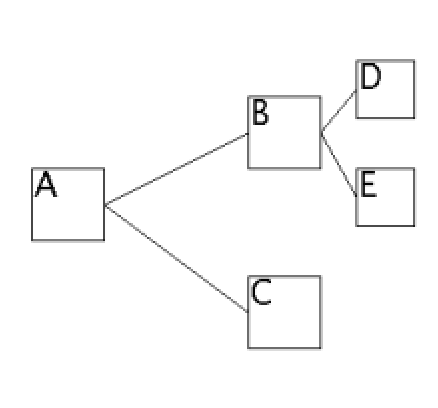
\includegraphics{d1start.ps}}\\%
b)\fbox{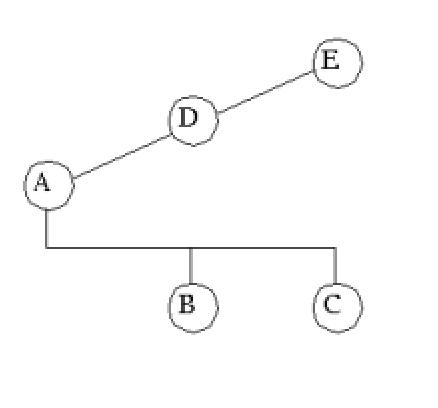
\includegraphics{d1end.ps}}\\%
c)\fbox{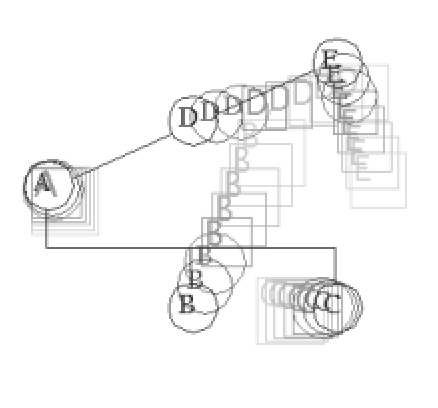
\includegraphics{composite.ps}}
% 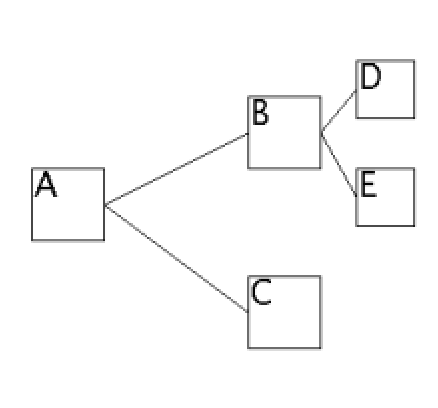
\includegraphics[width=\textwidth]{d1start.ps}
\vskip 3cm
\caption{
Example images drawn using the Vob library.
a), b) Two different views of the same ``objects'', showing
different relations between them.
When these two images are in sequence, it is difficult to see the
relationships between the objects.
c) An automatically generated animation sequence between the
two images. 
The animation of the B/W images is schematically shown here
by superimposing the single frames drawn by the Vob library
and graying out the earlier frames.
\label{fig-simple-vobs}
\label{figsimplevobs}
}
\end{figure}



\subsection{A Medium-Level Representation}

In order for for the Vob system to be able to generate the animation
in Fig.~\ref{fig-simple-vobs} without requiring the views to participate
in the process, it is obvious that the views have to provide the Vob
system with some kind of representation of their output. The design
of this representation is a key element of the Vob system.

A low-level representation, such as ``{\it 
draw a box at (50, 50, 100, 100), draw
a line at...}'' does not contain enough information for the kinds
of enhancements we are looking for.
On the other hand, a high-level representation 
such as a widget tree
would be too specific
to a particular kind of view, making it difficult or impossible
to create a simple, general mapping from one scene to another.
This would force the views to know about each other and the Vob system
to know about the specifics of the views, which is contrary to our goal of
showing animations between decoupled views.

The Vob system is a compromise between these two extremes: a medium-level
representation.
Instead of the high-level view issuing low-level graphic commands,
it places medium-level visible objects --- Vobs --- 
into a 2-D scene 
which in turn issue the graphics
commands when the scene is rendered.
Each Vob is associated with a {\em key},
using which it is possible to identify
Vobs of different types and different views with each other.
From the point of view of the Vob system, the key is an abstract entity
for which only the ``equals'' relation is relevant (this can be 
extended; see the section on Referential Media below).

As user interface elements,
the Vobs are on a different level than e.g.~widgets. 
First, the 2-D scene is {\em not} reused between frames:
it is on the level of a single keyframe.
Second, a scrollable list of elements is a widget, whereas
the elements of the list would be a natural choice for Vobs.
However, Vobs are also hierarchical, as expained below; a Vob
may contain a complete scene, so the whole list may be a Vob as well.

\subsection{Relationship between Vobs and Model-View-Controller}

\begin{figure}[bt!]
\fbox{\includegraphics[width=7.5cm]{vob_mvc.eps}}
\caption{An illustration of the relationship between Vobs and
the Model-View-Controller framework.
The Views pass parts of the Model along to the Vob layer, which is
then able to use this information for visual enhancements without
requiring the Views to know each other.
\label{figvobuml}
}
\end{figure}

The MVC (Model-View-Controller) framework\cite{krasner88cookbook} 
is often used in 
graphical user interfaces. 
There is an interesting relationship between this model and the Vob system:
the keys in the Vob objects are generally related to the MVC Model,
being either parts of it or identifiers for parts of it.

In a sense, the Vob pattern is about recognizing that parts
of the model are usually associated to distinct visible objects
on the display by views and allowing views to express this
association.

\subsection{Details: the Object Structure}

Our prototype Vob library has several classes, of which
\vob\ and \vobscene\ are the fundamental interfaces.
\vob\ is an abstract class which can be implemented by 
the views' helper classes; basically, the implementation
needs to know how to draw itself in a given region on screen
(using a {\tt java.awt.Graphics} object).
One important public field in \vob\ is the \key, which is
the key used for identifying different \vob s with each other.

The \vobscene class, on the other hand, is implemented by the Vob system.
The different views place \vob s
into \vobscene s, giving the \vobscene\ the coordinates and depth.
The \vobscene s are then able to interpolate
between each other smoothly, using the \key\ field of \vob,
requesting each \vob\ to draw itself at the interpolated coordinates
(on some graphics platforms, display lists may be used to optimize
this process).
Connections between different views are built by traversing \vobscene s
and connecting \vob s with similar keys.

The views can optionally be decoupled from the 
different implementations of \vob s for representing
a certain kind of object by using a factory pattern
in order to allow even more flexibility.

Returning to Figure \ref{fig-simple-vobs},which shows two different views
showing different relations between
the same abstract ``objects'' A-E, we note that
the important point is that the views and the Vobs are
decoupled from each other through the \vobscene\ and \vob\ APIs:
\begin{itemize}
\item The two views can be programmed separately, without any need
    for the views to know each other. The only connection between
    the views is that both render their result into a 
    \vobscene\ using implementations 
    of \vob\ using the same \key s from
    the underlying model for the ``object'' A-E.
\item The \vob\ objects
    that draw the ``objects'' in the two different views
    are of different classes, with no need to know each other.
\item The \vob\ objects that 
    do not have a counterpart with the same key
    in the other \vobscene\ (or whose \key\ is nil)
    appear in the final frame. It would also be possible to smoothly blend
    them in, but whether this is appropriate would depend on the
    nature of the view and the role of the \vob\ in the view.
    Here, the lines between A-E are keyless \vob s and
    because they represent connections, it is more appropriate
    to only draw them in the final frame.
\end{itemize}

\subsection{Animation/Morphing}

It is important to realize that the goal
of the Vob library is not to animate a single type of view
in the best possible way; applying animations in such contexts 
is discussed elsewhere, e.g.~in
\cite{lasseter87principles,chang-animation-cartoons}
the principles of traditional cartoon animation are applied to
computers. 
Instead, our goal is to come up with a system that
helps human perception when animating between different, completely
independent views
in most or all cases 
{\em with very little or no extra work} from the designer and the implementor
of the application.

Accordingly, the basic animation mode of the system is
linear interpolation between the Vobs with the same keys
in different keyframes; this is what is shown in Fig.~\ref{fig-simple-vobs}.

Despite the simplicity, the linear animation from one view to another 
is powerful:
When the user is shown an animation of such as the one 
in Fig.~\ref{fig-simple-vobs},
the relationship between the objects in 
the two different views is immediately clear.

In Fig.~\ref{fig-simple-vobs},
the squares change into circles in the middle of the motion.
This is the intended behaviour and is achieved by choosing which
\vobscene's \vob s are used to render the interpolated frame.
The idea is that 
the human eye will easier associate the two different forms with each
other due to the same direction and velocity of motion (however,
we have not performed user tests on this).

Of course, it is desirable to have the system be extensible so that
it is possible to specify the behaviour more accurately where
this is desired, e.g.~between certain Vob or view types.

The accurate timing of the animation is beyond the scope
of this paper; 
The Vob system
simply knows how to draw a scene interpolated a given amount
between the given scenes.
An interesting topic for further research is allowing the VobScene
to request the Vobs to draw themselves at different levels of detail.
Some work on such systems has been done, 
see e.g.~\cite{funkhouser93adaptive,bederson00jazz}.


\subsection{Connections between views}

Animation is not the only way to utilize the key field in Vobs.
When multiple views are shown side by side, it would be 
interesting to have some way of indicating when the same ``objects''
appear in both views.
This idea has been explored 
by Nelson\cite{as-we-will-think,ted-xanalogical-strcture-needed} 
for a long time:
it is already present in the earliest mockups for multiple-window
environments.

With Vobs, it is possible to do this --- again --- without requiring
any special steps from the views aside from setting meaningful
values for the key fields in Vobs. 
The Vobs with the same keys can be identified and connected by
code that is independent of the views.

The Sections on the File Browser and Referential Media below
show examples of this.

% \subsection{Efficiency}
% 
% The question of efficiency is important in interactive applications.
% The algorithms for the operations described in this article
% can be made efficient. 
% Depth-sorting a $N$-Vob 
% VobScene is at worst $O(N \log N)$. 
% Building the index to the Vobs based on the keys can be implemented
% using hashtables in $O(N)$ time, as can be the matching of two VobScenes
% using the hashtables, assuming that each Vob as $O(1)$ matching Vobs.
% For Referential Media, a different index based on the spans in the vob
% keys must be built. This can be done using interval trees
% in $O(N \log N)$ time.
% 
% In practice, the current prototype is able to match two XXX-\vob \vobscene s
% in XXX ms and after that to perform animation at XXX fps on
% a XXX (XXX fps if all graphics operations are ignored)


\section{GZIGZAG --- VOBS AND FOCUS+CONTEXT}

Our main example, and in fact the project that the Vob concept was
originally created for, is GZigZag.
It was realized only later that vobs can be useful in a more general setting.

GZigZag is a libr\'e implementation of Ted Nelson's ZigZag 
design\cite{zigzag-presentation,zigzag-welcome}.
In ZigZag, all data is represented as {\em cells} and connections
between cells along {\em dimensions}.
Dimensions are fully orthogonal to each other, so any cell
can be connected to any other cell. 
This structure, which emphasizes
the interconnectivity of information, is (naturally) ideally
suited for the Vob concept since the ultimate goal is that {\em all}
information is represented by cells in the same structure.
Because of this, the cells function well as Vob keys.

Figure \ref{figvanishing} shows three examples of different views
of a GZigZag structure.
These views are all focus+context\cite{fc-fisheye,fc-taxonomy} views,
meaning that there is one cell which is the {\em focus}, the center
of the view, and the surrounding cells are shown in a smaller scale.

Using the Vob system for the views and its linear interpolation
allows a greater degree of freedom than the usual way in which
focus+context views seem to be implemented:
in e.g.~the cone-tree\cite{robertson91cone} or 
hyperbolic view\cite{lamping96hyperbolic},
the animation is accomplished by smooth dependency of the position
of the elements from the parameters.
This means that the views must be designed so that all positions can
be reached on the continuous parameter manifold --- a relatively
difficult task in general. 
Switching between different views smoothly is impossible in this 
framework.

The Vob system, on the other hand, abandons the continuity of the views
and simply performs linear interpolation between keyframes.
This technique makes the resulting animations somewhat cruder, 
but on the other hand much flexibility is gained.
Programming new views is simple since they only need to place
the Vobs corresponding to the cells into the VobScene and
animation when moving the focus is filled in automatically.
For ZigZag,
this type of approach is doubly desirable, since the ZigZag space
cannot be evenly spread on two dimensions, neither Euclidean nor
hyperbolic, as would be required by certain types of fisheye views.

% For views such as these, the default linear interpolation of the Vob
% system seems to subjectively work very well; however, we have not
% yet perfomed any usability testing on this system.

\begin{figure}[tb!]
a)
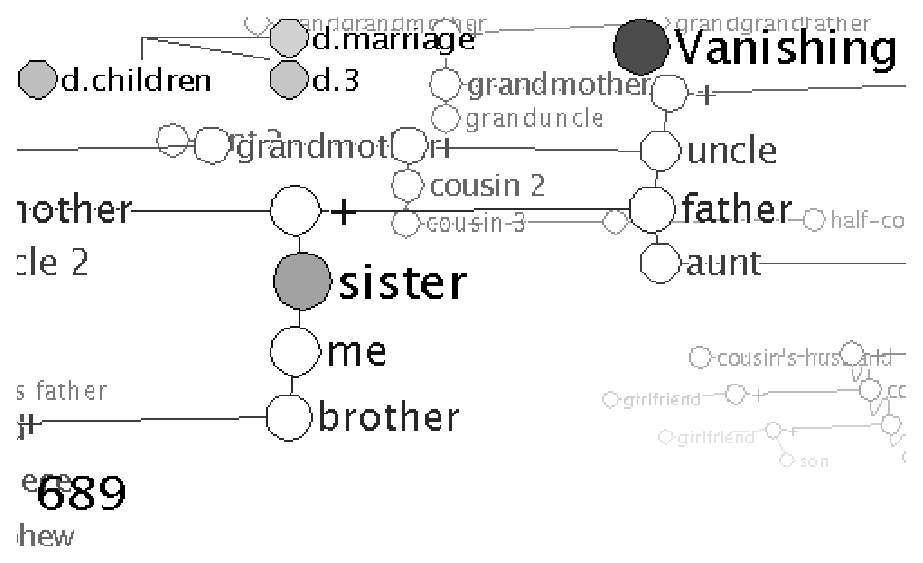
\includegraphics[width=7.5cm]{ZZPic1.eps}\vskip 0.3cm
b)
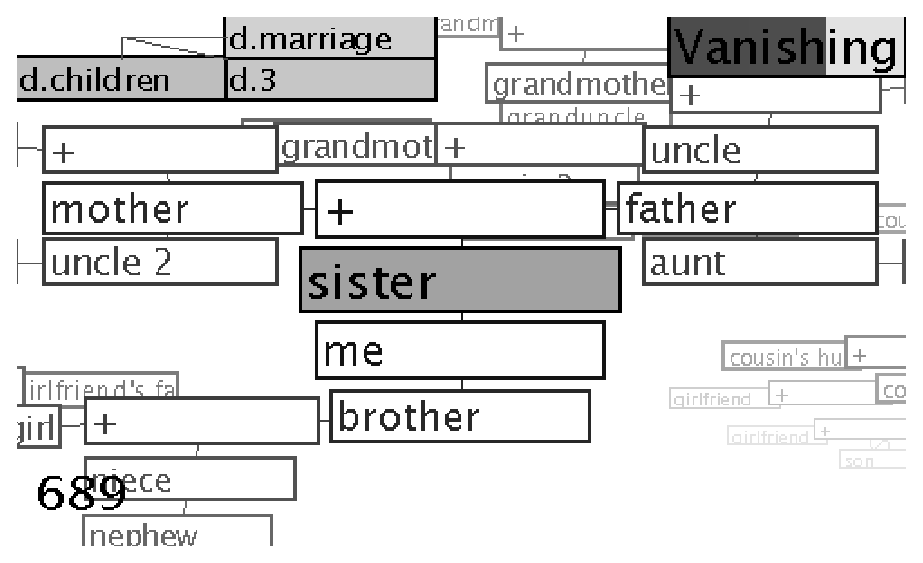
\includegraphics[width=7.5cm]{ZZPic2.eps}\vskip 0.3cm
c)
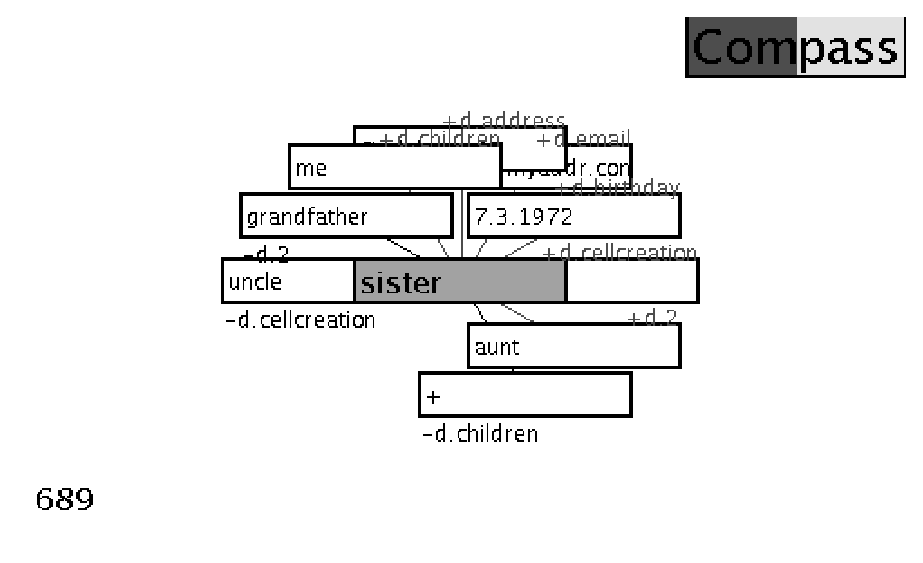
\includegraphics[width=7.5cm]{ZZPic3.eps}\vskip 0.3cm
\caption{
Some GZigZag views implemented using an older version of the Vob library.
a) The Vanishing view. This is a simple focus+context view
taking advantage of the depth-sorting provided by the Vob library.
The default animation using linear interpolation works well with this view.
b) Another of GZigZag's
focus+context views, the Compass view, 
with the cursor on the same cell as in a). 
The Vob animation (unfortunately not showable on paper)
allows the user to see ``what went where''
and reorient easily to the new configuration.
c) The Vanishing view drawn using a different Vob for cells.
The Vobs are created using a factory object so the visual representation
of cells can be changed without changing the view.
\label{figvanishing}
}
\end{figure}

\section{FILE BROWSER}

One common example of a model from which a large number of objects is 
shown in 
different views is the file system. Files are not only shown in many different
arrangements, also you could say that when a file is opened in an application,
it is simply shown in a different view.

%At the same time, file browsers are a good example for the problem the vob
%system attempts to solve. \benja{We damn well need a cite for the claims
%made here, or we might have to move them out again. But it's so central,
%I wouldn't know how to argue for the vobbed file browser without this!}

Common file browsers sort the files by different criteria like name and
size, and allow different views like the ``large icon'' and ``small icon''
views of Microsoft Windows' Explorer, or the ``symbol'' 
and ``list'' views of the
Macintosh Finder. When the view is changed, it is not easy to see where
the files from the previous view have gone. 
The users need to re-orient themselves by rereading the file names.

Using the vob system, animation of the files 
``flying into place''
(interpolated from their old to their new position) is generated
automatically. 
Also, when a file or icon is opened, current operating systems usually show a
little animation indicating the new window is a ``bigger representation''
of the file. The vob system can interpolate the file's icon to grow into the
window showing the file's contents. Of course this is nothing new, but the
vob system gives this automatically, without any extra effort.

% It appears that there are two important cases here, the first one
% being changing the
% sorting criteria for files. As, for big directories, a lot of files 
% move into a different arrangement in this case, there is a lot of animation
% in different directions; it is not immediately clear what went where, because
% there are too many files which changed places. Still, the overall motion
% becomes clear, and if one can usually follow a single file to its new
% place. 
% The second case is changing the view, e.g.
% from Window's ``big icon'' to ``small icon'' view. Here, the ordering of files
% remains the same, but the beginning of the rows of files is different.
% Changing to the ``list'' view, which layouts the files in columns instead of
% rows, is another example of this.
% 
% In the currently popular
% systems, again, it is hard to see where the files from the
% former view have ended up. In a filebrowser using the vob system, all the
% files animate in a similar manner, and it seems that the animation shows quite
% clearly what happened to the view. A special case is re-sizing the window:
% when on a row or column there is space for more files after re-sizing, the
% files are layouted differently; the vob system shows how the layouts
% relate to each other, the common systems don't.

Additionally, the Vob system makes it simple 
to show connections between the same files
shown in different parts of the display.

A proof-of-concept filebrowser is shown in Fig~\ref{figFB}.
Although we have not done any usability testing on this,
it seems that the animation does help in understanding {\em how} the view
changed.

\begin{figure}[bt!]
\fbox{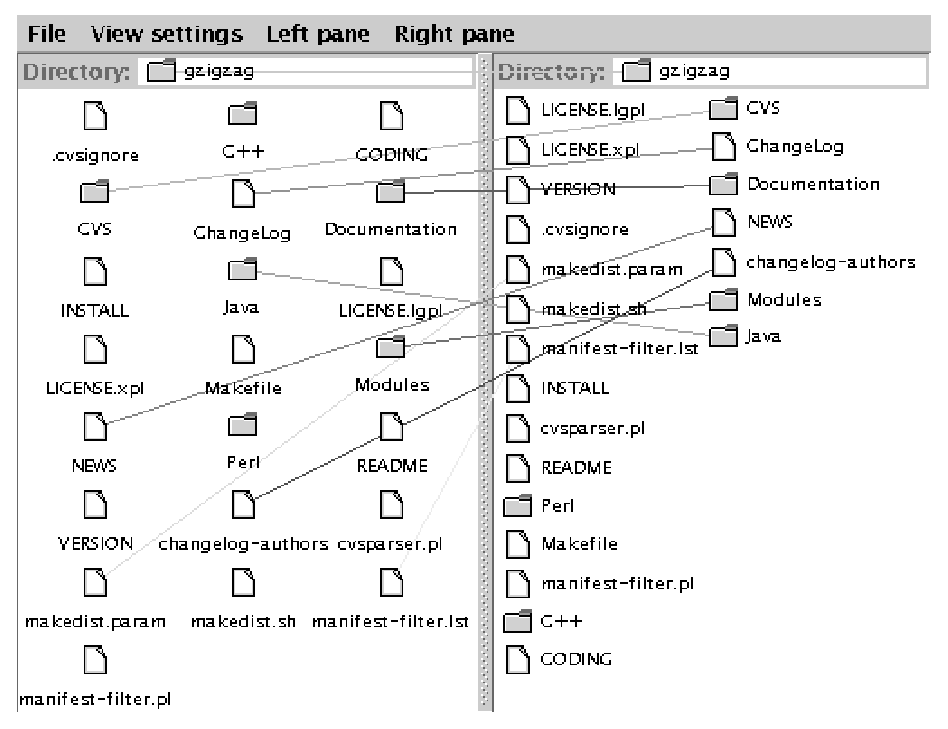
\includegraphics[width=7.5cm]{FileBrowserPic.eps}}
\caption{XXX
\label{figFB}
}
\end{figure}

The filebrowser is written combining Swing components with Vobs.
There are some special tricks to this:
Showing connections between different views 
which are located in different Swing components requires drawing
the connections across component boundaries, something that is not expected
by the common component systems. 
Furthermore, when an object from the model
appears first in one, then in another of the components (for example, after
dragging\&dropping it), an animation should show it moving from one component
to the other; this requires vobs to be drawn above the individual components,
as well. 
In the file browser demo, we create a
container component in which we place all components between which we show
connections. Inside the container component, we put {\em vob area} components,
which do not draw anything by themselves, but are used to determine the
region inside the container component's \vobscene\ into which
their view's vobs are placed into. 
When these components are moved or resized, the container's
\vobscene\ is refreshed, showing an animation to the new arrangement.
This approach does not support overlapping subcomponents; for that,
a more intricate approach is needed.

%  created; rather, we would use a special kind of vob holding a pointer to
% a component, and drawing itself by drawing that component. (Inlining 
% lightweight Java components in a scene graph has been done 
% n the Jazz toolkit\ref{bederson00jazz}.)
% This would allow us to generate animation between different arrangements of
% components, for example when a window has been resized. This could also be
% used to solve the problem of the approach described above, because vobs
% could be placed on the same depth as their vob area. However, a system
% like this hasn't been built yet.


\section{VOBS AND REFERENTIAL MEDIA}

In this Section, we discuss an important extension of the basic system
presented and used above.
The essential ingredient in the Vob system is the idea 
of identifying different visible objects in different views
representing the same underlying ``object''
with each other.
Different objects representing
e.g.~the same file are detected in order to 
allow visual enhancements. 

In the basic Vob framework, objects
and object equality is used for identity.
However (this is why we have used the quotes around ``object'' in 
this article), this is not the only possible way of identifying 
keys.

Below, we first discuss a different, more fine-grained
framework for identity pertaining to continuous media such as
text: the Xanadu media model, 
or referential media \cite{ted-xanalogical-structure-needed}
and after that we discuss its use in the Vob system.

\subsection{The Xanadu Media Model: Referential Media}

In the dominant paradigm, text and other media are treated as
sequences of numbers -- simply the content, with no reference to the
context. The Xanadu media model is based on a different approach:
when any human-entered piece of media enters the system, it obtains
a permanent identifier. 
One important feature of these identifiers is that they are
easy to split down to the level of single units --- in text, characters.
The permanent identifiers are called {\em spans}: a span refers
to a single, contiguous block of the entered media.

The same piece of media is always referred to through
the same identifier, so even after a piece of text has been cut\&pasted
into another document, its original source is traceable.
In the Xanadu model, including copies of (actually references to) 
the same piece of media in different documents is called {\em transclusion},
and forms an implicit link between the document.
Due to the above property of being able to split the references, the copies
need not be of the whole document but simply any part of it.

\begin{figure}[bt!]
\fbox{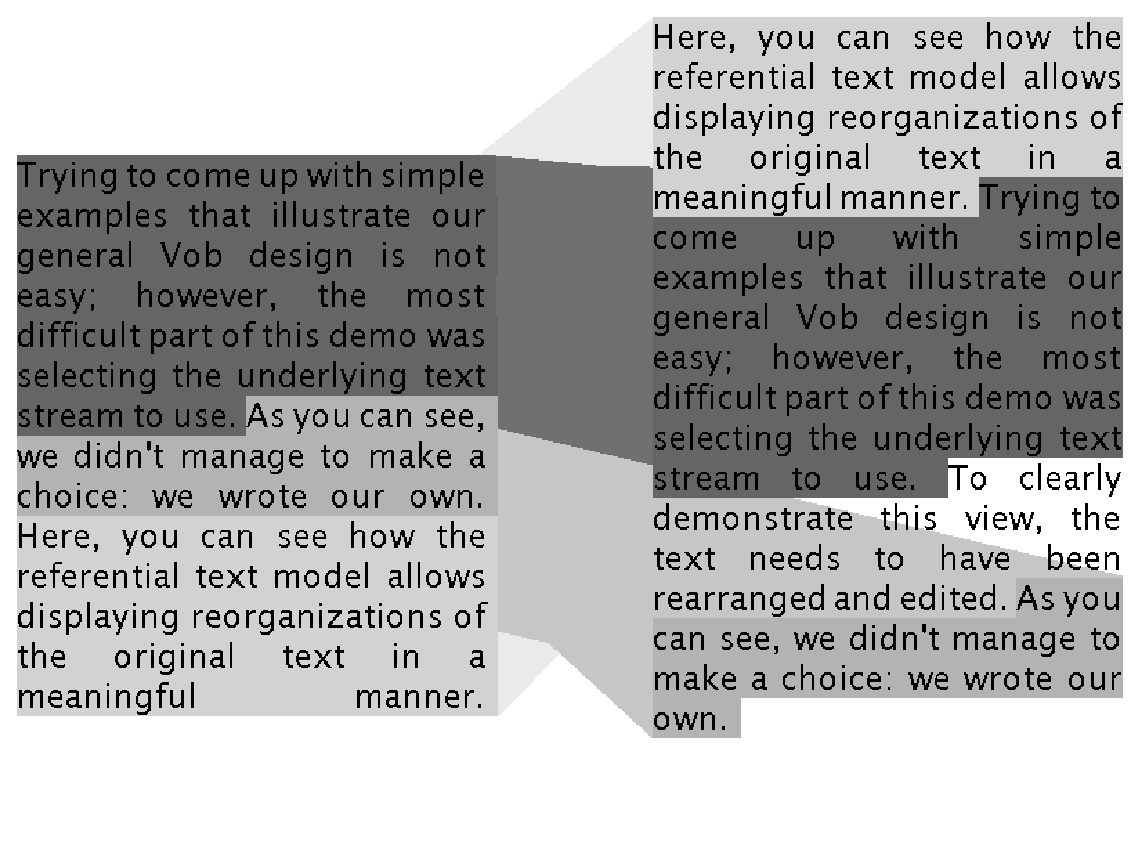
\includegraphics[width=7.5cm]{RefTextPic.eps}}
\caption{XXX
\label{figRefMed}
}
\end{figure}

\subsection{Spans as Vob Keys}

\begin{figure*}
\vskip 10cm
\caption{
\label{figspans}
Referential text in Vobs.
Two different text views,
showing two different versions of the same text.
The text that is the same 
in the views is connected by beams.
Note that this is {\helvixb not} 
simply a visual version of the Unix {\tt diff}
utility: the blocks of text that have been reorganized are still
connected, not just by an artificially computed least edit distance.
The Xanadu identity of the text is used.
}
\end{figure*}


The main consideration in using Xanadu spans as Vob keys
is the identity relationship. With plain object equality,
whole Vobs are always identified with other whole Vobs.
With spans, however, the overlap can be partial. 
This affects the animation and interconnection since
only a part of a given Vob must be connected with or animated to
a part of another Vob; this can be solved by subclassing 
\vob\ with a class which is able to provide the region 
intersecting a certain span on request.

Because of this, 
animating and connecting Vobs that contain spans does require
specialized code. 
However, several different strategies to connect and animate vobs
can be independently combined and applied to the \vobscene s,
so this does not lead to a significant complication in the basic model.

An example view produced by the Vob library is shown in Fig.~\ref{figspans}.

%If we want to show referential media using vobs, we face the problem that
%different views may show overlapping, but not identical media spans.
%Suppose we show two versions of a text document side-by-side. A vob may
%represent a whole sentce in one of the documents, but one word from this
%sentence can be transcluded to the other text. In this case, we want to show
%a connection between the two instances of the word, even though that's only
%a part of the sentence contained in the first vob. XXX

There are also other technical details beyond the scope
of this article, related for example
to the desire to have a single, continuous beam for parallel
sequences of vobs, and the use of GZigZag cells that contain spans
as keys. 
We refer the reader to our prototype implementation for 
a more complete exposition of these issues.


\section{AVAILABILITY OF THE PROTOTYPE IMPLEMENTATION}

Our prototype implementation of
the Vob library in pure Java
is free software, distributed under the LGPL license.
It is currently distributed as a part of GZigZag but the implementation
is wholly independent: the package {\tt org.gzigzag.vob} which
implements the Vob library does not contain any references to  
other {\tt org.gzigzag} packages.
The source code 
is available through {\tt http://gzigzag.org}; the Vob library 
is in the directory {\tt src/vob}. 

The prototype implementation contains some features which have not
been discussed in this article, such as color fogging for depth cues
(the effect can be seen in Fig.~\ref{figvanishing}).

\section{CONCLUSIONS}

We have presented the Vob framework which supports pervasive animation
between pluggable different views of the same data.

Our Vob approach shares some goals with 
Zoomable user interfaces\cite{bederson00jazz}, 
trying to get rid of the rigid widget-based approach.

However, contrary 
to the scene graph approach in ZUIs, the Vob system does not
enforce any global structure on the different views: the Vob
library is in this sense a lower-level API.



Now, \benja{Drop that ``now''!} animation and 
connectivity {\em per se}\/ are not novel ideas;


\tjl{VERY IMPORTANT. We have to explicitly say what is NEW}
animations have long been an important part of the field of computing
\nakki{XXX ref. e.g. tron movie!}
\cite{lasseter87principles}.
However, animation 
is usually achieved through continuously modifying some parameter 
in the view and redrawing, e.g.~in systems such as 
the hyperbolic browser\cite{lamping96hyperbolic} and 
XXX,
or by explicitly constructing the animation in the view, as in
code\cite{hudson93animation}.

\tjl{cone-tree, cam-tree, other fisheye views etc}.

Effectivity of using animation in UIs is discussed e.g. in
\cite{lasseter87principles,chang-animation-cartoons,chimera-tocs-animation}.

What is new is that we are aiming towards pervasive animation


\nakki{XXX REFERENCES THAT DISCUSS THESE SOMEHOW}


\benja{What comes after the conclusion? The references, obviously. So the
references discuss the vob system? Hm, that suggests that our ideas aren't
novel enough after all.}
The rest of the article discusses the Vob system,
which is an implementation 
of these enhancements in a way which 
attempts to
complicate the programming tasks
the least possible amount and also be efficient enough for use in real
systems.


\unfin

Incrementality - persistent / half-persistent data structs for vobscenes

Draw only changed rectangle

Janne: vob's not a widget, anyone can write one.

\fin

% The taps of Berlage\cite{berlage92taps} are a somewhat similar
% construction on the Controller side of the Model-View-Controller,
% similar in the sense that the Model is seen through a different


\section{ACKNOWLEDGMENTS}

The Vob system was developed in the GZigZag project, which
is a collaboration
with Ted Nelson.

We would like to thank Janne V. Kujala and Antti-Juhani Kaijanaho
for discussions.

% \bibliographystyle{abbrv}
\bibliography{gzigzag}

\end{document}
